\documentclass[onecolumn,unpublished]{quantumarticle}
\usepackage{amsmath}
\usepackage{amssymb}
\usepackage{amsthm}
\usepackage{amsfonts}
\usepackage[caption=false]{subfig}
\usepackage[colorlinks]{hyperref}
\usepackage[all]{hypcap}
\usepackage{tikz}
\usepackage{color,soul}
\usepackage[section]{placeins}
\usepackage[utf8]{inputenc}
\usepackage{capt-of}
\usepackage{multirow}
\usepackage{tabularx}
\usepackage{multicol}
\usepackage[numbers]{natbib}

\theoremstyle{definition}
\newtheorem{definition}{Definition}[section]
\theoremstyle{definition}
\newtheorem{theorem}{Theorem}[section]
\theoremstyle{definition}
\newtheorem{lemma}{Lemma}[section]

\newcommand{\hide}[1]{}

% use placeins for subsection also
\makeatletter
\AtBeginDocument{%
  \expandafter\renewcommand\expandafter\subsection\expandafter{%
    \expandafter\@fb@secFB\subsection
  }%
}
\makeatother

% Default fixed font does not support bold face
\DeclareFixedFont{\ttb}{T1}{txtt}{bx}{n}{12} % for bold
\DeclareFixedFont{\ttm}{T1}{txtt}{m}{n}{12}  % for normal

% Custom colors
\usepackage{color}
\definecolor{deepblue}{rgb}{0,0,0.5}
\definecolor{deepred}{rgb}{0.6,0,0}
\definecolor{deepgreen}{rgb}{0,0.5,0}

\usepackage{listings}

% Python style for highlighting
\newcommand\pythonstyle{\lstset{
language=Python,
basicstyle=\ttfamily,
otherkeywords={self,controlled_by,with,Mod,Quint,LookupTable},
keywordstyle=\bfseries\color{deepblue},
commentstyle=\color{gray},
emph={measure,__init__},
emphstyle=\bfseries\color{deepblue},
stringstyle=\color{deepgreen},
showstringspaces=false
}}


% Python environment
\lstnewenvironment{python}[1][]
{
\pythonstyle
\lstset{#1}
}
{}

\renewcommand\thesection{\arabic{section}}

\newcommand{\eq}[1]{\hyperref[eq:#1]{Equation~\ref*{eq:#1}}}
\renewcommand{\sec}[1]{\hyperref[sec:#1]{Section~\ref*{sec:#1}}}
\DeclareRobustCommand{\app}[1]{\hyperref[app:#1]{Appendix~\ref*{app:#1}}}
\newcommand{\fig}[1]{\hyperref[fig:#1]{Figure~\ref*{fig:#1}}}
\newcommand{\tbl}[1]{\hyperref[tbl:#1]{Table~\ref*{tbl:#1}}}
\newcommand{\theoremref}[1]{\hyperref[theorem:#1]{Theorem~\ref*{theorem:#1}}}
\newcommand{\definitionref}[1]{\hyperref[definition:#1]{Theorem~\ref*{definition:#1}}}

\newcommand{\cgate}[1]{*+<.6em>{#1} \POS ="i","i"+UR;"i"+UL **\dir{-};"i"+DL **\dir{-};"i"+DR **\dir{-};"i"+UR **\dir{-},"i" \cw}
\newcommand{\igate}[1]{*+<.6em>{#1} \POS ="i","i"+UR;"i"+UL **\dir{-};"i"+DL **\dir{-};"i"+DR **\dir{-};"i"+UR **\dir{-},"i"}
\newcommand{\imultigate}[2]{*+<1em,.9em>{\hphantom{#2}} \POS [0,0]="i",[0,0].[#1,0]="e",!C *{#2},"e"+UR;"e"+UL **\dir{-};"e"+DL **\dir{-};"e"+DR **\dir{-};"e"+UR **\dir{-},"i"}
\newcommand{\ighost}[1]{*+<1em,.9em>{\hphantom{#1}}}

\newcommand{\lenexp}{{n_e}}
\newcommand{\devoff}{{\delta_{\text{off}}}}
\newcommand{\gexp}{{g_{\text{exp}}}}
\newcommand{\gmul}{{g_{\text{mul}}}}
\newcommand{\gsep}{{g_{\text{sep}}}}
\newcommand{\gpad}{{g_{\text{pad}}}}
\newcommand{\distone}{{d_1}}
\newcommand{\disttwo}{{d_2}}
\newcommand{\productreg}{x}
\newcommand{\workreg}{y}

\newcommand{\pluseq}{\mathrel{+}=}
\newcommand{\minuseq}{\mathrel{-}=}
\newcommand{\timeseq}{\mathrel{\ast}=}

%    Q-circuit version 2
%    Copyright (C) 2004  Steve Flammia & Bryan Eastin
%    Last modified on: 9/16/2011
%
%    This program is free software; you can redistribute it and/or modify
%    it under the terms of the GNU General Public License as published by
%    the Free Software Foundation; either version 2 of the License, or
%    (at your option) any later version.
%
%    This program is distributed in the hope that it will be useful,
%    but WITHOUT ANY WARRANTY; without even the implied warranty of
%    MERCHANTABILITY or FITNESS FOR A PARTICULAR PURPOSE.  See the
%    GNU General Public License for more details.
%
%    You should have received a copy of the GNU General Public License
%    along with this program; if not, write to the Free Software
%    Foundation, Inc., 59 Temple Place, Suite 330, Boston, MA  02111-1307  USA

% Thanks to the Xy-pic guys, Kristoffer H Rose, Ross Moore, and Daniel Müllner,
% for their help in making Qcircuit work with Xy-pic version 3.8.  
% Thanks also to Dave Clader, Andrew Childs, Rafael Possignolo, Tyson Williams,
% Sergio Boixo, Cris Moore, Jonas Anderson, and Stephan Mertens for helping us test 
% and/or develop the new version.

\usepackage[color]{xy}
\UseCrayolaColors
\xyoption{matrix}
\xyoption{frame}
\xyoption{arrow}
\xyoption{arc}

\usepackage{ifpdf}
\ifpdf
\else
\PackageWarningNoLine{Qcircuit}{Qcircuit is loading in Postscript mode.  The Xy-pic options ps and dvips will be loaded.  If you wish to use other Postscript drivers for Xy-pic, you must modify the code in Qcircuit.tex}
%    The following options load the drivers most commonly required to
%    get proper Postscript output from Xy-pic.  Should these fail to work,
%    try replacing the following two lines with some of the other options
%    given in the Xy-pic reference manual.
\xyoption{ps}
\xyoption{dvips}
\fi

% The following resets Xy-pic matrix alignment to the pre-3.8 default, as
% required by Qcircuit.
\entrymodifiers={!C\entrybox}

%\newcommand{\bra}[1]{{\left\langle{#1}\right\vert}}
%\newcommand{\ket}[1]{{\left\vert{#1}\right\rangle}}
    % Defines Dirac notation. %7/5/07 added extra braces so that the commands will work in subscripts.
\newcommand{\qw}[1][-1]{\ar @{-} [0,#1]}
\newcommand{\eqw}[1][-1]{\ar @{-} @[Red] [0,#1]}
    % Defines a wire that connects horizontally.  By default it connects to the object on the left of the current object.
    % WARNING: Wire commands must appear after the gate in any given entry.
\newcommand{\qwx}[1][-1]{\ar @{-} [#1,0]}
    % Defines a wire that connects vertically.  By default it connects to the object above the current object.
    % WARNING: Wire commands must appear after the gate in any given entry.
\newcommand{\cw}[1][-1]{\ar @{=} [0,#1]}
    % Defines a classical wire that connects horizontally.  By default it connects to the object on the left of the current object.
    % WARNING: Wire commands must appear after the gate in any given entry.
\newcommand{\cwx}[1][-1]{\ar @{=} [#1,0]}
    % Defines a classical wire that connects vertically.  By default it connects to the object above the current object.
    % WARNING: Wire commands must appear after the gate in any given entry.
\newcommand{\gate}[1]{*+<.6em>{#1} \POS ="i","i"+UR;"i"+UL **\dir{-};"i"+DL **\dir{-};"i"+DR **\dir{-};"i"+UR **\dir{-},"i" \qw}
\newcommand{\eboxgate} [1]{*+<.6em>{#1} \POS ="i","i"+UR;"i"+UL **[red]\dir{-};"i"+DL **[red]\dir{-};"i"+DR **[red]\dir{-};"i"+UR **[red]\dir{-},"i" \eqw}
\newcommand{\circgate}[1]{*+<0.6em>[o][F-]{#1} \eqw}
\newcommand{\ecircgate}[1]{*+<0.6em>[o][F-:red]{#1} \eqw}
\newcommand{\filtergt}[1]{\eboxgate{\scriptscriptstyle{#1}}}
\newcommand{\idealdec}{*+<1.2em>{\phantom{*}} \POS ="i","i"+UL;"i"+DL **[red]\dir{-};"i"+R **[red]\dir{-};"i"+UL **[red]\dir{-},"i" \eqw}

    % Boxes the argument, making a gate.
\newcommand{\meter}{*=<1.8em,1.4em>{\xy ="j","j"-<.778em,.322em>;{"j"+<.778em,-.322em> \ellipse ur,_{}},"j"-<0em,.4em>;p+<.5em,.9em> **\dir{-},"j"+<2.2em,2.2em>*{},"j"-<2.2em,2.2em>*{} \endxy} \POS ="i","i"+UR;"i"+UL **\dir{-};"i"+DL **\dir{-};"i"+DR **\dir{-};"i"+UR **\dir{-},"i" \qw}
    % Inserts a measurement meter.
    % In case you're wondering, the constants .778em and .322em specify
    % one quarter of a circle with radius 1.1em.
    % The points added at + and - <2.2em,2.2em> are there to strech the
    % canvas, ensuring that the size is unaffected by erratic spacing issues
    % with the arc.
\newcommand{\measure}[1]{*+[F-:<.9em>]{#1} \qw}
    % Inserts a measurement bubble with user defined text.
\newcommand{\measuretab}[1]{*{\xy*+<.6em>{#1}="e";"e"+UL;"e"+UR **\dir{-};"e"+DR **\dir{-};"e"+DL **\dir{-};"e"+LC-<.5em,0em> **\dir{-};"e"+UL **\dir{-} \endxy} \qw}
    % Inserts a measurement tab with user defined text.
\newcommand{\measureD}[1]{*{\xy*+=<0em,.1em>{#1}="e";"e"+UR+<0em,.25em>;"e"+UL+<-.5em,.25em> **\dir{-};"e"+DL+<-.5em,-.25em> **\dir{-};"e"+DR+<0em,-.25em> **\dir{-};{"e"+UR+<0em,.25em>\ellipse^{}};"e"+C:,+(0,1)*{} \endxy} \qw}
\newcommand{\emeasureD}[1]{*{\xy*+=<0em,.1em>{#1}="e";"e"+UR+<0em,.25em>;"e"+UL+<-.5em,.25em> **[red]\dir{-};"e"+DL+<-.5em,-.25em> **[red]\dir{-};"e"+DR+<0em,-.25em> **[red]\dir{-};{"e"+UR+<0em,.25em>\ellipse{}};"e"+C:,+(0,1)*{} \endxy} \qw}
    % Inserts a D-shaped measurement gate with user defined text.
\newcommand{\multimeasure}[2]{*+<1em,.9em>{\hphantom{#2}} \qw \POS[0,0].[#1,0];p !C *{#2},p \drop\frm<.9em>{-}}
    % Draws a multiple qubit measurement bubble starting at the current position and spanning #1 additional gates below.
    % #2 gives the label for the gate.
    % You must use an argument of the same width as #2 in \ghost for the wires to connect properly on the lower lines.
\newcommand{\multimeasureD}[2]{*+<1em,.9em>{\hphantom{#2}} \POS [0,0]="i",[0,0].[#1,0]="e",!C *{#2},"e"+UR-<.8em,0em>;"e"+UL **\dir{-};"e"+DL **\dir{-};"e"+DR+<-.8em,0em> **\dir{-};{"e"+DR+<0em,.8em>\ellipse^{}};"e"+UR+<0em,-.8em> **\dir{-};{"e"+UR-<.8em,0em>\ellipse^{}},"i" \qw}
    % Draws a multiple qubit D-shaped measurement gate starting at the current position and spanning #1 additional gates below.
    % #2 gives the label for the gate.
    % You must use an argument of the same width as #2 in \ghost for the wires to connect properly on the lower lines.
\newcommand{\control}{*!<0em,.025em>-=-<.2em>{\bullet}}
    % Inserts an unconnected control.
\newcommand{\controlo}{*+<.01em>{\xy -<.095em>*\xycircle<.19em>{} \endxy}}
    % Inserts a unconnected control-on-0.
\newcommand{\ctrl}[1]{\control \qwx[#1] \qw}
    % Inserts a control and connects it to the object #1 wires below.
\newcommand{\ctrlo}[1]{\controlo \qwx[#1] \qw}
    % Inserts a control-on-0 and connects it to the object #1 wires below.
\newcommand{\targ}{*+<.02em,.02em>{\xy ="i","i"-<.39em,0em>;"i"+<.39em,0em> **\dir{-}, "i"-<0em,.39em>;"i"+<0em,.39em> **\dir{-},"i"*\xycircle<.4em>{} \endxy} \qw}
    % Inserts a CNOT target.
\newcommand{\qswap}{*=<0em>{\times} \qw}
    % Inserts half a swap gate.
    % Must be connected to the other swap with \qwx.
\newcommand{\multigate}[2]{*+<1em,.9em>{\hphantom{#2}} \POS [0,0]="i",[0,0].[#1,0]="e",!C *{#2},"e"+UR;"e"+UL **\dir{-};"e"+DL **\dir{-};"e"+DR **\dir{-};"e"+UR **\dir{-},"i" \qw}
    % Draws a multiple qubit gate starting at the current position and spanning #1 additional gates below.
    % #2 gives the label for the gate.
    % You must use an argument of the same width as #2 in \ghost for the wires to connect properly on the lower lines.
\newcommand{\ghost}[1]{*+<1em,.9em>{\hphantom{#1}} \qw}
    % Leaves space for \multigate on wires other than the one on which \multigate appears.  Without this command wires will cross your gate.
    % #1 should match the second argument in the corresponding \multigate.
\newcommand{\push}[1]{*{#1}}
    % Inserts #1, overriding the default that causes entries to have zero size.  This command takes the place of a gate.
    % Like a gate, it must precede any wire commands.
    % \push is useful for forcing columns apart.
    % NOTE: It might be useful to know that a gate is about 1.3 times the height of its contents.  I.e. \gate{M} is 1.3em tall.
    % WARNING: \push must appear before any wire commands and may not appear in an entry with a gate or label.
\newcommand{\gategroup}[6]{\POS"#1,#2"."#3,#2"."#1,#4"."#3,#4"!C*+<#5>\frm{#6}}
    % Constructs a box or bracket enclosing the square block spanning rows #1-#3 and columns=#2-#4.
    % The block is given a margin #5/2, so #5 should be a valid length.
    % #6 can take the following arguments -- or . or _\} or ^\} or \{ or \} or _) or ^) or ( or ) where the first two options yield dashed and
    % dotted boxes respectively, and the last eight options yield bottom, top, left, and right braces of the curly or normal variety.  See the Xy-pic reference manual for more options.
    % \gategroup can appear at the end of any gate entry, but it's good form to pick either the last entry or one of the corner gates.
    % BUG: \gategroup uses the four corner gates to determine the size of the bounding box.  Other gates may stick out of that box.  See \prop.

\newcommand{\rstick}[1]{*!L!<-.5em,0em>=<0em>{#1}}
    % Centers the left side of #1 in the cell.  Intended for lining up wire labels.  Note that non-gates have default size zero.
\newcommand{\lstick}[1]{*!R!<.5em,0em>=<0em>{#1}}
    % Centers the right side of #1 in the cell.  Intended for lining up wire labels.  Note that non-gates have default size zero.
\newcommand{\ustick}[1]{*!D!<0em,-.5em>=<0em>{#1}}
    % Centers the bottom of #1 in the cell.  Intended for lining up wire labels.  Note that non-gates have default size zero.
\newcommand{\dstick}[1]{*!U!<0em,.5em>=<0em>{#1}}
    % Centers the top of #1 in the cell.  Intended for lining up wire labels.  Note that non-gates have default size zero.
\newcommand{\Qcircuit}{\xymatrix @*=<0em>}
    % Defines \Qcircuit as an \xymatrix with entries of default size 0em.
\newcommand{\link}[2]{\ar @{-} [#1,#2]}
    % Draws a wire or connecting line to the element #1 rows down and #2 columns forward.
\newcommand{\pureghost}[1]{*+<1em,.9em>{\hphantom{#1}}}
    % Same as \ghost except it omits the wire leading to the left. 
%%%%%%%%%%%%%%%%%%%%%%%%%%%%%%%%%%%%%%%%%%%%%%%%%%%%%%%%%%%%%%%%%%%%%%%%%%%%%%%%%%%%%%%%%%
\newcommand{\multiprepareC}[2]{*+<1em,.9em>{\hphantom{#2}}\save[0,0].[#1,0];p\save !C
  *{#2},p+RU+<0em,0em>;+LU+<+.8em,0em> **\dir{-}\restore\save +RD;+RU **\dir{-}\restore\save
  +RD;+LD+<.8em,0em> **\dir{-} \restore\save +LD+<0em,.8em>;+LU-<0em,.8em> **\dir{-} \restore \POS
  !UL*!UL{\cir<.9em>{u_r}};!DL*!DL{\cir<.9em>{l_u}}\restore}
   % Draws a multiple qubit reverse-D-shaped preparation gate starting at the current position and spanning #1 additional gates below.
   % #2 gives the label for the gate.
   % You must use an argument of the same width as #2 in \pureghost for the wires to connect properly on
% the lower lines.
\newcommand{\prepareC}[1]{*{\xy*+=+<.5em>{\vphantom{#1\rule{0em}{.1em}}}*\cir{l^r};p\save*!L{#1} \restore\save+UC;+UC+<.5em,0em>*!L{\hphantom{#1}}+R **\dir{-} \restore\save+DC;+DC+<.5em,0em>*!L{\hphantom{#1}}+R **\dir{-} \restore\POS+UC+<.5em,0em>*!L{\hphantom{#1}}+R;+DC+<.5em,0em>*!L{\hphantom{#1}}+R **\dir{-} \endxy}}
   % Inserts a reverse-D-shaped preparation gate with user defined text.
\newcommand{\poloFantasmaCn}[1]{{{}^{#1}_{\phantom{#1}}}}


\begin{document}
\title{Windowed quantum arithmetic using QROM lookups}

\date{\today}
\author{Craig Gidney}
\email{craiggidney@google.com}
\affiliation{Google Inc., Santa Barbara, California 93117, USA}

\begin{abstract}
We describe a technique, which we refer to as ``windowing", for optimizing quantum arithmetic circuits based on using QROM lookups to iterate over groups of qubits instead of individual qubits.
We show that windowing lowers the cost of several quantum arithmetic tasks involving multiplications and classical constants at register sizes relevant in practice.
Windowed constructions can be nested, though there is a cost, which we demonstrate by constructing a windowed modular exponentiation with nested windowed modular multiplications.
\end{abstract}

\maketitle




\section{Introduction}
\label{sec:introduction}

Physical qubits are noisy \cite{schroeder2009dram,Bare13,Kim2014}, and quantum error correction is expensive \cite{fowler2012surfacecodereview, campbell2018constraintsatisfaction}.
Because of this, we expect fault tolerant quantum computers to be billions of times less efficient than classical computers, at least on an operation-by-operation basis.
This creates a surprising situation, where replacing one quantum operation with a million classical operations is actually an {\em optimization}.

In this paper, we are interested in cases where a quantum algorithm could perform less work if a register storing a classical function of some small number of qubits was available.
When this occurs, it can be beneficial to brute-force evaluate the function by encoding it into a QROM lookup \cite{babbush2018} (hereafter ``table lookup").
For example, when starting a modular exponentiation, looking up the final result of the first twenty iterations of the repeated squaring process is significantly more efficient than actually performing twenty controlled modular multiplications (despite the fact that producing the lookup circuit requires classically computing a million possible products).

The paper is organized as follows.
\sec{introduction} describes the structure of the paper.
In \sec{background}, we review background information on performing table lookups over classical data addressed by quantum data.
In \sec{results}, we provide pseudo-code using  table lookups to accelerate several quantum arithmetic tasks related to multiplications involving classical constants.
Finally, in \sec{conclusion} we summarize our contributions and discuss their implications.



\section{Background: table lookups}
\label{sec:background}

A table lookup is an operation that retrieves data from a classical table addressed by a quantum register.
It performs the operation $\sum_{j=0}^{L-1} |j\rangle|0\rangle \rightarrow \sum_{j=0}^{L-1} |j\rangle|T_j\rangle$, where $T$ is a classically precomputed table with $L$ entries.
In \fig{lookup} we relay a construction that performs this operation with a Toffoli count of $L-1$, independent of the number of bits in each entry, from \cite{babbush2018}.

It is possible to compute a table lookup in $O(WL/k + k)$ Toffolis, where $W$ is the output size of the lookup and $k$ is a freely chosen parameter \cite{low2018qrom}.
Unfortunately, doing so requires $O(Wk)$ dirty ancillae.
The lookups we are performing in this paper are most beneficial when $W$ is large, and so we avoid this optimization when computing lookups.
However, when uncomputing a lookup, an eager measurement trick makes these optimizations applicable \cite{berry2019qubitization}.

\begin{figure}
\centering
\resizebox{\textwidth}{!}{
\Qcircuit @R=0.7em @C=0.5em {
&\multigate{2}{\text{Input }a}           &\qw& &&&&&&\ctrlo{3} &\qw      &\qw       &\qw      &\qw      &\qw       &\qw      &\qw       &\qw       &\qw      &\qw      &\qw       &\qw      &\qw      &\qw      &\qw       &\qw       &\qw      &\qw      &\qw       &\qw      &\qw       &\qw       &\qw      &\qw      &\qw       &\qw      &\qw      &\ctrl{3} &\qw     &\\
&       \ghost{\text{Input }a}           &\qw& &&&&&&\qw       &\ctrlo{3}&\qw       &\qw      &\qw      &\qw       &\qw      &\qw       &\qw       &\qw      &\qw      &\qw       &\qw      &\ctrl{3} &\qw      &\ctrlo{3} &\qw       &\qw      &\qw      &\qw       &\qw      &\qw       &\qw       &\qw      &\qw      &\qw       &\qw      &\ctrl{3} &\qw      &\qw     &\\
&       \ghost{\text{Input }a}           &\qw& &&&&&&\qw       &\qw      &\ctrlo{3} &\qw      &\qw      &\qw       &\ctrl{3} &\qw       &\ctrlo{3} &\qw      &\qw      &\qw       &\ctrl{3} &\qw      &\qw      &\qw       &\ctrlo{3} &\qw      &\qw      &\qw       &\ctrl{3} &\qw       &\ctrlo{3} &\qw      &\qw      &\qw       &\ctrl{3} &\qw      &\qw      &\qw     &\\
&       \ctrl{4}   \qwx                  &\qw& &&&&&&\ctrl{1}  &\qw      &\qw       &\qw      &\qw      &\qw       &\qw      &\qw       &\qw       &\qw      &\qw      &\qw       &\qw      &\qw      &\ctrl{1} &\qw       &\qw       &\qw      &\qw      &\qw       &\qw      &\qw       &\qw       &\qw      &\qw      &\qw       &\qw      &\qw      &\ctrl{1} &\qw     &\\
&                                        &   & &&&&&&          &\ctrl{1} &\qw       &\qw      &\qw      &\qw       &\qw      &\ctrl{1}  &\qw       &\qw      &\qw      &\qw       &\qw      &\ctrl{1} &\targ    &\ctrl{1}  &\qw       &\qw      &\qw      &\qw       &\qw      &\ctrl{1}  &\qw       &\qw      &\qw      &\qw       &\qw      &\ctrl{1} &\qw      &        &\\
&                                        &   & &&=&&&&          &         &\ctrl{1}  &\qw      &\ctrl{1} &\qw       &\ctrl{1} &\targ     &\ctrl{1}  &\qw      &\ctrl{1} &\qw       &\ctrl{1} &\qw      &         &          &\ctrl{1}  &\qw      &\ctrl{1} &\qw       &\ctrl{1} &\targ     &\ctrl{1}  &\qw      &\ctrl{1} &\qw       &\ctrl{1} &\qw      &         &        &\\
&                                        &   & &&&&&&          &         &          &\ctrl{6} &\targ    &\ctrl{6}  &\qw      &          &          &\ctrl{6} &\targ    &\ctrl{6}  &\qw      &         &         &          &          &\ctrl{6} &\targ    &\ctrl{6}  &\qw      &          &          &\ctrl{6} &\targ    &\ctrl{6}  &\qw      &         &         &        &\\
&\multigate{5}{\oplus\text{Lookup }T_a}     &\qw& &&&&&&\qw       &\qw      &\qw       &\targ^?  &\qw      &\targ^?   &\qw      &\qw       &\qw       &\targ^?  &\qw      &\targ^?   &\qw      &\qw      &\qw      &\qw       &\qw       &\targ^?  &\qw      &\targ^?   &\qw      &\qw       &\qw       &\targ^?  &\qw      &\targ^?   &\qw      &\qw      &\qw      &\qw     &\\
&       \ghost{\oplus\text{Lookup }T_a}     &\qw& &&&&&&\qw       &\qw      &\qw       &\targ^?  &\qw      &\targ^?   &\qw      &\qw       &\qw       &\targ^?  &\qw      &\targ^?   &\qw      &\qw      &\qw      &\qw       &\qw       &\targ^?  &\qw      &\targ^?   &\qw      &\qw       &\qw       &\targ^?  &\qw      &\targ^?   &\qw      &\qw      &\qw      &\qw     &\\
&       \ghost{\oplus\text{Lookup }T_a}     &\qw& &&&&&&\qw       &\qw      &\qw       &\targ^?  &\qw      &\targ^?   &\qw      &\qw       &\qw       &\targ^?  &\qw      &\targ^?   &\qw      &\qw      &\qw      &\qw       &\qw       &\targ^?  &\qw      &\targ^?   &\qw      &\qw       &\qw       &\targ^?  &\qw      &\targ^?   &\qw      &\qw      &\qw      &\qw     &\\
&       \ghost{\oplus\text{Lookup }T_a}     &\qw& &&&&&&\qw       &\qw      &\qw       &\targ^?  &\qw      &\targ^?   &\qw      &\qw       &\qw       &\targ^?  &\qw      &\targ^?   &\qw      &\qw      &\qw      &\qw       &\qw       &\targ^?  &\qw      &\targ^?   &\qw      &\qw       &\qw       &\targ^?  &\qw      &\targ^?   &\qw      &\qw      &\qw      &\qw     &\\
&       \ghost{\oplus\text{Lookup }T_a}     &\qw& &&&&&&\qw       &\qw      &\qw       &\targ^?  &\qw      &\targ^?   &\qw      &\qw       &\qw       &\targ^?  &\qw      &\targ^?   &\qw      &\qw      &\qw      &\qw       &\qw       &\targ^?  &\qw      &\targ^?   &\qw      &\qw       &\qw       &\targ^?  &\qw      &\targ^?   &\qw      &\qw      &\qw      &\qw     &\\
&       \ghost{\oplus\text{Lookup }T_a}     &\qw& &&&&&&\qw       &\qw      &\qw       &\targ^?  &\qw      &\targ^?   &\qw      &\qw       &\qw       &\targ^?  &\qw      &\targ^?   &\qw      &\qw      &\qw      &\qw       &\qw       &\targ^?  &\qw      &\targ^?   &\qw      &\qw       &\qw       &\targ^?  &\qw      &\targ^?   &\qw      &\qw      &\qw      &\qw     &\\
&                                           &   & &&&&&&          &         &          &T_0      &         &T_1       &         &          &          &T_2      &         &T_3 &&&&&&T_4 &&T_5 &&&&T_6 &&T_7   &&&&&&\\
&&&&&&&&& &&& &&&&& &&&&&&& &&& && &&&   &&&&&&\\
}
}
    \caption{
        \label{fig:lookup}
        Table lookup circuit from \cite{babbush2018}.
        The lines emerging from and merging into other lines are AND computations and uncomputations (notation from \cite{gidney2018addition}); they are equivalent to Toffoli gates.
        If the control qubit is set and the address register contains the binary value $a$, then this circuit xors the $a$'th bitstring from a precomputed lookup table $T$ into the $W$ target qubits.
        The diagram is showing the case where $L=2^3$ and $W=6$.
        The question marks beside the CNOT targets indicate that the target should be omitted or included depending on a corresponding bit in $T$.
    }
\end{figure}

To uncompute a table lookup, start by measuring all of the output qubits in the X basis.
This will produce random measurement results, but the results will indicate which computational basis states of the address register need to be negated in order to complete the uncomputation.
Negating these states can be performed using a lookup over a smaller table with fewer output qubits.
And, because space was just conveniently made available by the measurements, there is significant available workspace.

Concretely, the phase negation task is performed by separating the address register into a low half and a high half.
A binary-to-unary conversion (see \fig{unary}) is performed on the low half, and then a table lookup addressed by the high half and targeting the low half is performed.
See \fig{unlookup} for a quantum circuit showing an overview of this process.

Because of the uncomputation optimization, the Toffoli count of uncomputing the lookup is $2\sqrt{L}$ instead of $L$.
Asymptotically negligible compared to the cost of computing the lookup.



\begin{figure}
\centering
\resizebox{!}{!}{
\Qcircuit @R=1em @C=0.75em {
& \multigate{2}{\text{Input }x}         &\qw && &&& &\qw&\qw                &\qw     &\ctrl{4}&\qw     &\qw     &\qw     &\qw     &\qw     &\qw     &\qw     &\\
&        \ghost{\text{Input }x}         &\qw && &&& &\qw&\qw                &\qw     &\qw     &\ctrl{4}&\ctrl{5}&\qw     &\qw     &\qw     &\qw     &\qw     &\\
&        \ghost{\text{Input }x}         &\qw && &&& &\qw&\qw                &\qw     &\qw     &\qw     &\qw     &\ctrl{5}&\ctrl{6}&\ctrl{7}&\ctrl{8}&\qw     &\\
&\imultigate{7}{\text{Init Unary }x}\qwx&\qw && &&& &   &\lstick{|0\rangle} &\targ   &\qswap  &\qswap  &\qw     &\qswap  &\qw     &\qw     &\qw     &\qw     \\
&       \ighost{\text{Init Unary }x}    &\qw && &&& &   &\lstick{|0\rangle} &\qw     &\qswap  &\qw     &\qswap  &\qw     &\qswap  &\qw     &\qw     &\qw     \\
&       \ighost{\text{Init Unary }x}    &\qw &&=&&& &   &\lstick{|0\rangle} &\qw     &\qw     &\qswap  &\qw     &\qw     &\qw     &\qswap  &\qw     &\qw     \\
&       \ighost{\text{Init Unary }x}    &\qw && &&& &   &\lstick{|0\rangle} &\qw     &\qw     &\qw     &\qswap  &\qw     &\qw     &\qw     &\qswap  &\qw     \\
&       \ighost{\text{Init Unary }x}    &\qw && &&& &   &\lstick{|0\rangle} &\qw     &\qw     &\qw     &\qw     &\qswap  &\qw     &\qw     &\qw     &\qw     \\
&       \ighost{\text{Init Unary }x}    &\qw && &&& &   &\lstick{|0\rangle} &\qw     &\qw     &\qw     &\qw     &\qw     &\qswap  &\qw     &\qw     &\qw     \\
&       \ighost{\text{Init Unary }x}    &\qw && &&& &   &\lstick{|0\rangle} &\qw     &\qw     &\qw     &\qw     &\qw     &\qw     &\qswap  &\qw     &\qw     \\
&       \ighost{\text{Init Unary }x}    &\qw && &&& &   &\lstick{|0\rangle} &\qw     &\qw     &\qw     &\qw     &\qw     &\qw     &\qw     &\qswap  &\qw     \\
}
}
    \caption{
        \label{fig:unary}
        Circuit for producing a unary register from a binary register, using $L$ Toffoli gates where $L$ is the length of the unary register (and $\lg L$ is the length of the binary register).
        The qubit at offset $k$ of the unary register is set if the binary register is storing $|k\rangle$.
        The ``Clear Unary" circuit can be performed by running this circuit in reverse, or by using a construction based on eager measurements followed by phase fixups.
    }
\end{figure}

\begin{figure}
\resizebox{\textwidth}{!}{
\Qcircuit @R=1em @C=0.75em {
  &\qw    &                 \qw&\qw &                               \ctrl{1} &\qw&&& &&&&&\qw    &          \qw       &\qw &     \qw&   \qw&                                     \qw&    \qw&\qw&\qw&               \qw&    \qw&                 \qw&                             \qw&     \qw&                    \ctrl{1}                  &     \qw&                                      \qw&\qw&\\
  &\qw {/}&          \qw       &\qw &       \multigate{1}{\text{Input }a}    &\qw&&& &&&&&\qw {/}&          \qw       &\qw &     \qw&   \qw&                                     \qw&\qw    &\qw&\qw&               \qw&\qw    &          \qw       &                             \qw&     \qw&                   \gate{\text{Input }a_0}    &     \qw&                                      \qw&\qw&\\
  &\qw {/}&\ustick{l}\qw       &\qw &              \ghost{\text{Input }a}    &\qw&&&=&&&&&\qw {/}&\ustick{l}\qw       &\qw &     \qw&   \qw&                                     \qw&\qw    &\qw&\qw&               \qw&\qw    &          \qw       &\gate{\text{Input }a_1}         &     \qw&                                       \qw\qwx&     \qw&             \gate{\text{Input }a_1}     &\qw&\\
  &\qw {/}&\ustick{\geq 2^l}\qw&\qw &        \gate{\text{Unlookup }D_{a}}\qwx& \rstick{\langle0|} \qw   &&& &&&&&\qw {/}&\ustick{\geq 2^l}\qw&\qw &\gate{H}&\meter&                                 \cw    &       &   &   &\lstick{|0\rangle}&\qw {/}&\ustick{2^l}     \qw&\gate{\text{Init Unary }a_1}\qwx&\gate{H}&        \gate{\oplus\text{Lookup }F_{a_0}}\qwx&\gate{H}&        \gate{\text{Clear Unary }a_1}\qwx& \rstick{\langle0|} \qw&    \\
  &       &                    &    &                                        &   &&& &&&&&       &                    &    &        &      &\igate{\text{Compute fixup table }F}\cwx&\cw {/}&\cw&\cw&               \cw&    \cw&                 \cw&                             \cw&     \cw& \cw\cwx&
}
}
    \caption{
        \label{fig:unlookup}
        Uncomputing a table lookup with address space size $L$ and a word size larger than $\sqrt{L}$.
        Has a Toffoli count and measurement depth of $O(\sqrt{L})$.
        Quadratically cheaper than computing the table lookup.
    }
\end{figure}




\section{Results: windowed arithmetic circuits}
\label{sec:results}

\subsection{Product addition}

A product addition operation performs $x \pluseq ky$.
We focus on the case where $k$ is a classical constant.

Normally an implementation of this operation would iterate over the bits of $k$, because this creates many small opportunities for optimization.
We instead start from an implementation iterating over the qubits of $y$ and performing quantum controlled additions:

\begin{python}
    def plus_equal_product(target: Quint, k: int, y: Quint):
        for i in range(len(y)):
            with control(y[i]):
                target[i:] += k
\end{python}

Adding $k$ into $x$ controlled by a qubit $q$ is equivalent to adding into $x$ the result of a table lookup with $q$ as the address, the value $0$ at address 0, and the value $k$ at address 1.
So the above code is equivalent to the following code:

\begin{python}
    def plus_equal_product(target: Quint, k: int, y: Quint):
        table = LookupTable([0, classical_factor])
        for i in range(len(quantum_factor)):
            target[i:] += table[quantum_factor[i]]
\end{python}

Instead of performing a lookup over one qubit, we can perform a lookup over many qubits.
That is to say, we can introduce windowing:

\begin{python}
    def plus_equal_product(target: Quint,
                           k: int,
                           y: Quint,
                           window: int):
        table = LookupTable([
            i*k
            for i in range(2**window)
        ])
        for i in range(0, len(quantum_factor), window):
            w = quantum_factor[i:i+window]
            target[i:] += table[w]
\end{python}

This windowed implementation of product addition has an asymptotic Toffoli count of $O(\frac{n}{w} (n + 2^w))$ where $w$ is the window size.
Setting the window size to $w=\lg n$, so that the table lookup is as expensive as the addition, achieves a Toffoli complexity of $O(n^2/\lg n)$.
A logarithmic factor improvement over the construction we started with.

We used Q\# to measure the cost of our windowed construction versus other constructions.
See \fig{product-add-costs}.
The estimation methodology is as follows.
We implemented all three constructions in Q\#, and then iterated over problem sizes while using the tracing simulator to count the number of Toffolis and the number of qubits.
We generated one random problem at each problem size, and fed it to all three constructions while checking that they each returned the correct result.
Note that we were not able to use the table lookup uncomputation optimization, because it was incompatible with Q\#'s Toffoli simulator.

We amortized the resulting numbers in order to make differences easier to see.
To estimate the physical spacetime numbers we assumed a code distance of 31, a control system reaction time of 10 microseconds, and that ``time optimal computing" \cite{fowler2012time} was being used.


\subsection{Multiplication}

A multiplication operation performs $x \timeseq k$ where $k$ is odd.
Because qubits later in $x$ cannot affect qubits earlier in $x$, this operation can be implemented by iterating over $x$, from most significant qubit to least significant qubit, performing controlled additions targeting the rest of the register:

\begin{python}
    def times_equal(target: Quint, k: int):
        assert k % 2 == 1
        for i in range(len(target))[::-1]:
            with control(target[i]):
                target[i+1:] += k >> 1
\end{python}

As in the previous subsection, we can rewrite the controlled addition into a lookup addition, and then window the lookup.
However, there is a complication introduced by the fact that qubits within a window need to operate on each other.
To handle this, we split the inner-loop into two steps: adding the correct value into the rest of the register, and then recursively multiplying within the window.

\begin{python}
    def times_equal(target: Quint, k: int, window: int):
        assert k % 2 == 1  # Even factors aren't reversible.
        k %= 2**len(target)  # Normalize factor.
        if k == 1:
            return
        table = LookupTable([
            (j * k) >> window
            for j in range(2**window)
        ])
        for j in range(0, len(target), window)[::-1]:
            w = target[i:j+window]
            target[i+window:] += table[w]

            # Recursively fix up the window.
            times_equal_windowed(w, k, window=1)
\end{python}

The Toffoli complexity of this windowed multiplication is $O(\frac{n}{w} \cdot (n + 2^w + w^2))$.
If we set $w = \lg n$ then the Toffoli count is $O(n^2/\lg n)$.


\subsection{Modular product addition}

A modular product addition operation performs $x \pluseq k y \pmod{N}$.
We focus on the case where $k$ and $N$ are classical constants.
We require that $x$, $y$, and $k$ are all non-negative and less than $N$.

Modular product addition is identical to product addition, except that we need to use a modular addition in the inner loop, we need to fold the position factor $2^i$ into the table lookup, and we need to ensure the table lookup returns a value modulo $N$:

\begin{python}
    def plus_equal_product_modulo(target: ModQuint,
                                  k: int,
                                  y: Quint,
                                  window: int):
        N = target.modulus
        for i in range(0, len(quantum_factor), window):
            w = quantum_factor[i:i+window]
            table = LookupTable([
                classical_factor*k*2**i % N
                for k in range(2**window)
            ])
            target += table[w]
\end{python}

See also \fig{multiply-add}, which generalizes this code to the case where $k$ is a function of a small number of qubits.
This code achieves a Toffoli count of $O(\frac{n}{w} (n + 2^w))$ and, setting $w=\lg n$ as usual, the Toffoli complexity is $O(n^2/\lg n)$.


\subsection{Modular multiplication}

A modular multiplication operation performs $x \timeseq k \pmod{N}$, where $k$ has a multiplicative inverse modulo $N$.
We focus on the case where $k$ and $N$ are classical constants.

Modular multiplication is performed via a series of modular product additions \cite{zalka2006pure, haner2016factoring, gidney2017factoring}, and so this case reduces to the modular product addition case from the previous subsection.
See \fig{multiply}.

\begin{figure}
\centering
\resizebox{0.7\textwidth}{!}{
\Qcircuit @R=1em @C=0.75em {
 \\
 &\qw {/}&\ustick{n}\qw&\qw &\gate{\times k \pmod{N}}  &\qw&&&=&&&   &\qw {/}&\ustick{n}\qw&\gate{\text{Input a}}&\gate{+b(-k^{-1}) \pmod{N}}          &\qswap    &\qw\\
 &       &             &    &                          &   &&& &&&\lstick{|0\rangle}     &\qw {/}&\ustick{n}\qw&\gate{+ak \pmod{N}}       \qwx&\gate{\text{Input b}}\qwx&\qswap\qwx&\qw\\
 \\
}
}
    \caption{
        \label{fig:multiply}
        Modular multiplication decomposes into modular product additions.
    }
\end{figure}


\subsection{Modular exponentiation multiplication}

A modular exponentiation multiplication operation performs $x \timeseq k^e \pmod{N}$, where $k$ has a multiplicative inverse modulo $N$.
We focus on the case where $k$ and $N$ are classical constants.

Modular exponentiation multiplication is typically implemented using a series of controlled modular multiplications \cite{vedral1996arithmetic,zalka1998fast,haner2016factoring,gidney2017factoring}.
We can reduce the number of multiplications that are needed by iterate over small windows of the exponent, looking up the corresponding factor to multiply by for each one.
This also removes the need for the multiplications to be controlled, because the table lookup can evaluate to the factor 1 in cases where none of the exponent qubits are set.

There is a catch here.
Windowing over the exponent results in fewer modular multiplications, but the number being multiplied against is now quantum instead of classical.
At first glance, this seems to prevent us from applying windowing to the modular multiplications.
However, there is a solution to this problem: include the exponent qubits as parameters in the lookups within the modular multiplication, so that we can always look up the value relevant to the factor being multiplied by.
This produces code with two windowing parameters:

\begin{python}
    def times_equal_modular_exponentation(target: ModQuint,
                                          k: int,
                                          e: Quint,
                                          e_window: int,
                                          m_window: int):
        a = target
        b = alloc(ModQuint(len(target)))
        N = target.modulus
        assert modinv(k, N) is not None

        for i in range(0, len(e), e_window):
            exp_index = e[i:i+g]
            ks = [pow(base, 2**i * e, modulus)
                  for e in range(2**e_window)]
            ks_inv = [modinv(k, modulus) for k in ks]
    
            # Perform b += a * k (mod modulus).
            # Maps (x, 0) into (x, x*k).
            for j in range(0, len(a), m_window):
                mul_index = a[j:j + g]
                table = LookupTable(
                    [(k * f * 2**j) % modulus
                     for f in range(2**len(mul_index))]
                    for k in ks)
                b += table[exp_index, mul_index]
    
            # Perform a -= b * inv(k) (mod modulus).
            # Maps (x, x*k) into (0, x*k).
            for j in range(0, len(a), m_window):
                mul_index = b[j:j + g]
                table = LookupTable(
                    [(k_inv * f * 2**j) % modulus
                     for f in range(2**len(mul_index))]
                    for k_inv in ks_inv)
                a -= table[exp_index, mul_index]
    
            # Relabelling swap. Maps (0, x*k) into (x*k, 0).
            a, b = b, a

        # Xor swap result into correct register if needed.
        if a is not target:
            a ^= b
            b ^= a
            a ^= b
        qfree(b)
\end{python}

See also \fig{exponentiation}.
The Toffoli complexity of this code is $O(\frac{n_e n}{w_e w_m} (n + 2^{w_e + w_m}))$ where $n_e$ is the number of exponent qubits, $n$ is the register size, $w_e$ is the exponent windowing size, and $w_m$ is the multiplication windowing size.
For the same reason that square fences cover more area per perimeter than rectangular fences, it is best to use roughly even window sizes over the exponentiation and the multiplications.
Setting $w_e=w_m=\frac{1}{2}\lg n$ achieves a Toffoli complexity of $O(\frac{n_e n^2}{\lg^2 n})$.


\begin{figure}[h]
\resizebox{\textwidth}{!}{
\Qcircuit @R=1em @C=0.75em {
\\
&\qw&\qw&\multigate{5}{\text{Input }e}&\qw&\qw &&&&& &\qw&\qw&       \multigate{1}{\text{Input }e_{0:2}}&\qw&\qw&\qw&\\
&\qw&\qw&\ghost{\text{Input }e}&\qw&\qw &&&&& &\qw&\qw&              \ghost{\text{Input }e_{0:2}}&\qw&\qw&\qw&\\
&\qw&\qw&\ghost{\text{Input }e}&\qw&\qw &&&&& &\qw&\qw&\qw\qwx&       \multigate{1}{\text{Input }e_{2:4}}&\qw&\qw&\\
&\qw&\qw&\ghost{\text{Input }e}&\qw&\qw &&&=&& &\qw&\qw&\qw\qwx&              \ghost{\text{Input }e_{2:4}}&\qw&\qw&\\
&\qw&\qw&\ghost{\text{Input }e}&\qw&\qw &&&&& &\qw&\qw&\qw\qwx&\qw\qwx&       \multigate{1}{\text{Input }e_{4:6}}&\qw&\\
&\qw&\qw&\ghost{\text{Input }e}&\qw&\qw &&&&& &\qw&\qw&\qw\qwx&\qw\qwx&              \ghost{\text{Input }e_{4:6}}&\qw&\\
&{/}\qw&\ustick{n}\qw&\gate{\times k^e \pmod{N}}\qwx&\qw&\qw &&&&& &{/}\qw&\ustick{n}\qw&\gate{\times k^{2^0 e_{0:2}} \pmod{N}}\qwx& \gate{\times k^{2^2 e_{2:4}} \pmod{N}}\qwx& \gate{\times k^{2^4 e_{4:6}} \pmod{N}}\qwx&\qw&\\
\\
}
}
    \caption{
    \label{fig:exponentiation}
    A six-exponent-qubit modular exponentiation multiplication circuit performed using windowed arithmetic with an exponent window size of 2.
    The relevant exponent qubits have to be included as address qubits in lookups within the windowed modular product addition circuits, as seen in \fig{multiply-add}.
    }
\end{figure}

\begin{figure}[h]
\resizebox{\textwidth}{!}{
\Qcircuit @R=1em @C=0.75em {
 \\
 &\qw {/}&\ustick{w_e}\qw&\gate{\text{Input }e}         \qw    &\qw&& &&&&&&&\lstick{\text{exponent}}&\qw {/}&\ustick{w_e}\qw&\gate{\text{Input }e}                           \qw    &                     \qw    &\gate{\text{Input }e}                             \qw    &\qw &\dots &&\gate{\text{Input }e}                                                   \qw    &                     \qw    &\gate{\text{Input }e}                                                                 \qw    &\qw\\
 &\qw    &              \qw&\multigate{4}{\text{Input }a} \qw\qwx&\qw&& &&&&&&&\lstick{\text{in}_0}    &\qw    &          \qw&\multigate{1}{\text{Input }a_0}                 \qw\qwx&                     \qw    &\multigate{1}{\text{Input }a_0}                   \qw\qwx&\qw &\dots &&                                                                        \qw\qwx&                     \qw    &                                                                                  \qw\qwx&\qw\\
 &\qw    &              \qw&       \ghost{\text{Input }a} \qw    &\qw&& &&&&&&&\lstick{\text{in}_1}    &\qw    &          \qw&       \ghost{\text{Input }a_0}                 \qw    &                     \qw    &       \ghost{\text{Input }a_0}                   \qw    &\qw &\dots &&                                                                        \qw\qwx&                     \qw    &                                                                                  \qw\qwx&\qw\\
 &       &           \vdots&                                     &   && &&&&&&&\lstick{\vdots}         &       &             &                                                   \qwx&                            &                                                     \qwx&    &\ddots&&                                                                           \qwx&                            &                                                                                     \qwx&   \\
 &\qw    &              \qw&       \ghost{\text{Input }a} \qw    &\qw&& &&&&&&&\lstick{\text{in}_{m-2}}&\qw    &          \qw&                                                \qw\qwx&                     \qw    &                                                  \qw\qwx&\qw &\dots &&\multigate{1}{\text{Input }a_{\lceil m/g-1\rceil}}                      \qw\qwx&                     \qw    &\multigate{1}{\text{Input }a_{\lceil m/g-1 \rceil}}                               \qw\qwx&\qw\\
 &\qw    &              \qw&       \ghost{\text{Input }a} \qw    &\qw&& &&&&&&&\lstick{\text{in}_{m-1}}&\qw    &          \qw&                                                \qw\qwx&                     \qw    &                                                  \qw\qwx&\qw &\dots &&       \ghost{\text{Input }a_{\lceil m/g-1\rceil}}                      \qw    &                     \qw    &       \ghost{\text{Input }a_{\lceil m/g-1 \rceil}}                               \qw    &\qw\\
 &\qw {/}&\ustick{m}    \qw&                              \qw\qwx&\qw&& &&&&&&&\lstick{|0\rangle}      &\qw {/}&\ustick{m}\qw&\gate{\otimes \text{Lookup }a_0 k^e 2^0\pmod{N}}\qw\qwx&\gate{\text{Input }v}\qw    &\gate{\text{Unlookup } a_0 k^e 2^g \pmod{N}}\qw\qwx&\qw &\dots &&\gate{\otimes \text{Lookup } a_{\lceil m/g-1\rceil} k^e 2^{g \lceil m/g-1\rceil} \pmod{N}}\qw\qwx&\gate{\text{Input }v}\qw    &\gate{\text{Unlookup } a_{\lceil m/g-1\rceil} k^e 2^{g \lceil m/g - 1 \rceil} \pmod{N}}\qw\qwx&\qw\\
 &\qw {/}&\ustick{m}    \qw&\gate{+ak^e \pmod{N}}  \qw\qwx&\qw&& &&&&&&&\lstick{\text{out}}     &\qw {/}&\ustick{m}\qw&                                                \qw    &\gate{+v \pmod{N}}            \qw\qwx&                                                  \qw    &\qw &\dots &&                                                                        \qw    &\gate{+v \pmod{N}}            \qw\qwx&                                                                                  \qw    &\qw\\
 \\
}
}
    \caption{
        \label{fig:multiply-add}
        A modular product addition circuit using windowed arithmetic, where the factor to multiply by is derived from a small number of input qubits from an exponent in a modular exponentiation.
    }
\end{figure}

\begin{figure}
    \centering
    \resizebox{\linewidth}{!}{
        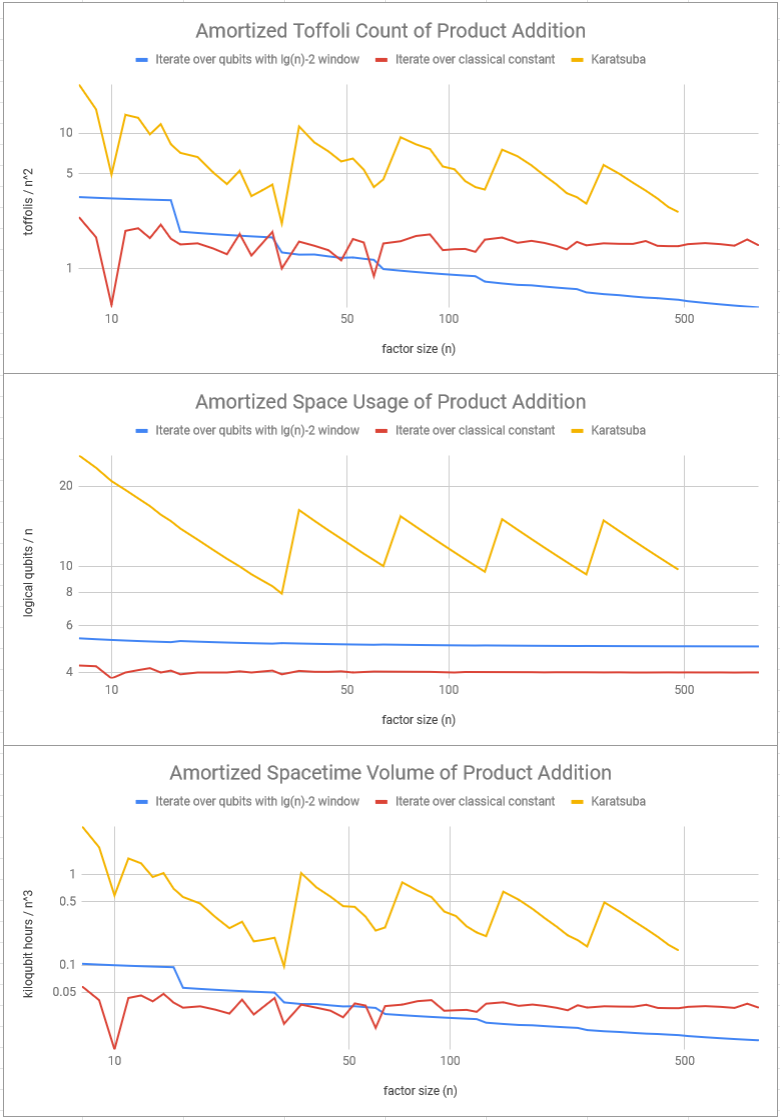
\includegraphics{assets/costs.png}
    }
    \caption{
        \label{fig:product-add-costs}
        Amortized costs of performing the operation $x \pluseq ky$ where $k$ is a classical constant using windowed arithmetic, iteration over the classical constant, and the Karatsuba multiplication procedure from \cite{gidney2019karatsuba}.
        Although the Karatsuba volume curve will eventually go below the windowed arithmetic volume curve, this does not happen until well past factor sizes that would be relevant in practice.
    }
\end{figure}


\section{Conclusion}
\label{sec:conclusion}

In this paper we introduced the concept of windowing, which uses small table lookups to optimize quantum arithmetic circuits.
We presented constructions using this technique for several multiplication tasks involving classical constants.
These constructions are asymptotically less efficient than using non-trivial multiplication algorithms (such as Karatsuba multiplication), but save log factors versus schoolbook multiplication and have good constant factors.
As a result, our windowed arithmetic constructions do very well at small register sizes.

Even at register sizes that would be used in Shor's algorithm, our constructions are more efficient than previous work.
This suggests that windowing will be a mainstay of quantum circuit construction.


\section{Acknowledgements}
We thank Adam Langley, Ilya Mironov, and Ananth Raghunathan for reading a draft of this paper and providing useful feedback which improved it.
We thank Austin Fowler, Martin Ekerå, and Johan Håstad for useful feedback and discussions.
We thank Hartmut Neven for creating an environment where this research was possible in the first place.

\bibliographystyle{plainnat}
\bibliography{refs}


\end{document}
